
\begin{frame}{‌مرتب‌سازی سریع}
\begin{itemize}\itemr
\item[-]
یکی از الگوریتم‌های مرتب‌سازی بسیار پر استفاده الگوریتم مرتب‌سازی سریع
\fn{1}{quicksort algorithm}
است.
\item[-]
این الگوریتم یک الگوریتم تقسیم و حل است. زمان اجرای آن در بدترین حالت
\ath{n^2}
است، اما در حالت میانگین در زمان
\ath{n \lg n}
اجرا می‌شود. این الگوریتم به حافظه اضافی نیاز ندارد.
\end{itemize}
\end{frame}


\begin{frame}{‌مرتب‌سازی سریع}
\begin{itemize}\itemr
\item[-]
برای مرتب‌سازی آرایه
\code{A[p:r]}
این الگوریتم از روش تقسیم و حل به صورت زیر استفاده می‌کند.
\item[۱.]
تقسیم : آرایهٔ
\code{A[p:r]}
به دو قسمت
\code{A[p:q-1]}
(قسمت پایین)
\fn{1}{low side}
و
\code{A[q+1:r]}
(قسمت بالا)
\fn{2}{high side}
تقسیم می‌شود به طوری که همه عناصر قسمت پایین از عنصر
\code{A[q]}
(عنصر محور)
\fn{3}{pivot}
کوچکتر یا برابرند و عناصر قسمت بالا از عنصر محور بزرگ‌ترند.
\item[۲.]
حل : الگوریتم مرتب‌سازی سریع برای دو زیر آرایه
\code{A[p:q-1]}
و
\code{A[q+1:r]}
فراخوانی می‌شود.
\item[۳.]
ترکیب : در این قسمت هیچ عملیاتی انجام نمی‌شود. از آنجایی که همه عناصر
\code{A[p:q-1]}
مرتب شده و کوچکتر یا مساوی
\code{A[q]}
هستند و همهٔ عناصر
\code{A[q+1:r]}
مرتب شده و بزرگتر از
\code{A[q]}
هستند، بنابراین کل آرایه
\code{A[p:r]}
مرتب شده است.
\end{itemize}
\end{frame}

\begin{frame}{‌مرتب‌سازی سریع}
\begin{itemize}\itemr
\item[-]
در تقسیم آرایه به دو قسمت پایین و بالا، فرض کنید قسمت کرمی رنگ در شکل زیر عناصری باشند که مقدار آنها از عنصر محوری x کمتر و قسمت آبی رنگ عناصری باشند که مقدار آنها از عنصر محوری بیشتر است.
\begin{figure}
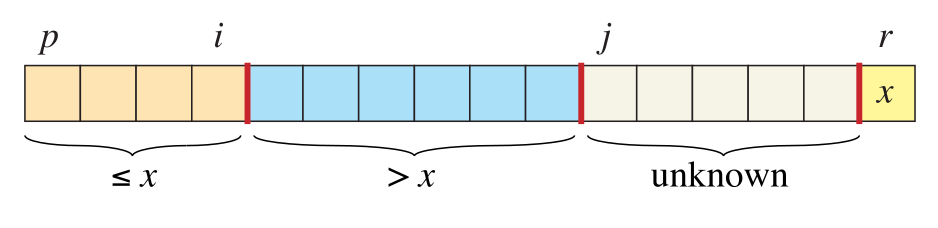
\includegraphics[width=0.7\textwidth]{figs/chap03/quicksort1}
\end{figure}
\end{itemize}
\end{frame}


\begin{frame}{‌مرتب‌سازی سریع}
\begin{itemize}\itemr
\item[-]
اندیس i مرز بین قسمت پایین و قسمت بالا را نگهداری می‌کند. توسط اندیس j عناصر آرایه یک به یک بررسی می‌شوند. در صورتی که مقدار آنها از عنصر محوری x کمتر باشد به صورت زیر به قسمت پایین منتقل می‌شوند و مرز قسمت پایین و بالا تغییر می‌کند، در غیر اینصورت قسمت در مکان خود نگه داشته می‌شوند.
\begin{figure}
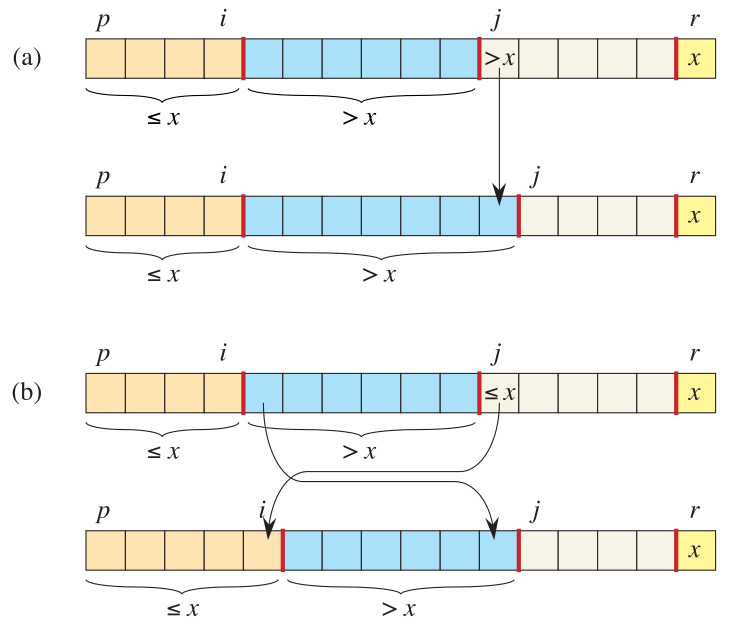
\includegraphics[width=0.5\textwidth]{figs/chap03/quicksort2}
\end{figure}
\end{itemize}
\end{frame}


\begin{frame}{‌مرتب‌سازی سریع}
\begin{itemize}\itemr
\item[-]
در شکل زیر نحوه اجرای الگوریتم تقسیم‌بندی نشان داده شده است. عنصر محور در اینجا برابر است با
\code{A[r]}.
\begin{figure}
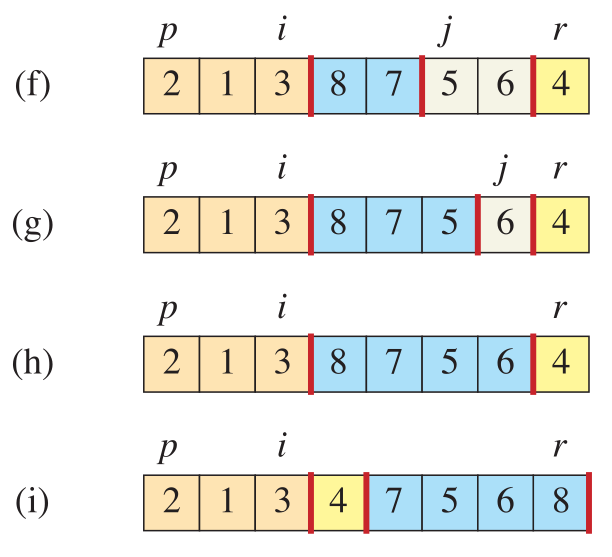
\includegraphics[width=0.4\textwidth]{figs/chap03/partition2}
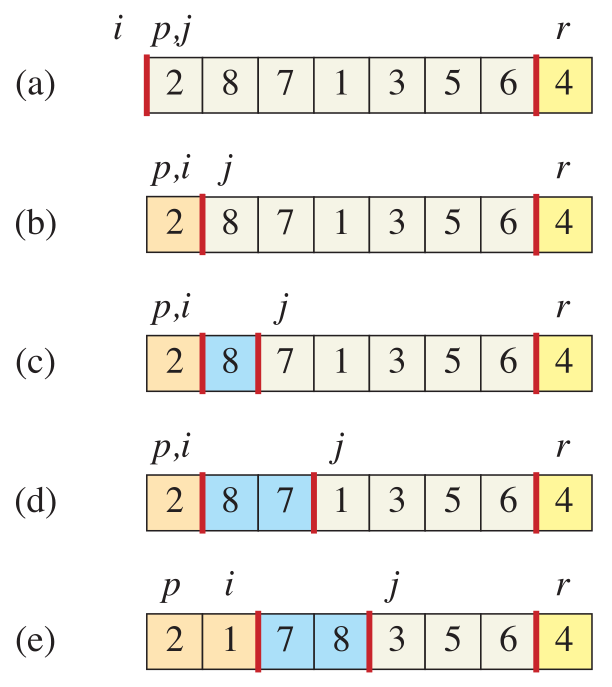
\includegraphics[width=0.4\textwidth]{figs/chap03/partition1}
\end{figure}
\end{itemize}
\end{frame}



\begin{frame}{‌مرتب‌سازی سریع}
\begin{itemize}\itemr
\item[-]
الگوریتم مرتب‌سازی سریع به صورت زیر است.
\begin{algorithm}[H]\alglr
  \caption{Quicksort} 
  \begin{algorithmic}[1]
   \Func{Quicksort}{A, p, r}
   \If{p < r}
           \LeftComment{Partition the subarray around the pivot, which ends up in A[q].}
           \State q = Partition (A, p, r)
           \State Quicksort (A, p, q-1) \LeftComment{recursively sort the low side}
           \State Quicksort (A, q+1, r) \LeftComment{recursively sort the high side}
    \EndIf                           
  \end{algorithmic}
  \label{alg:merge}
\end{algorithm}
\end{itemize}
\end{frame}


\begin{frame}{‌مرتب‌سازی سریع}
\begin{itemize}\itemr
\item[-]
الگوریتم تقسیم‌بندی
\fn{1}{partition}
باید عناصر آرایه را به گونه‌ای جابجا کند که همهٔ عناصر قسمت پایین از عنصر محور کوچک‌تر یا مساوی و عناصر قسمت بالا از عنصر محور بزرگ‌تر باشند.
\end{itemize}
\end{frame}


\begin{frame}{‌مرتب‌سازی سریع}
\begin{itemize}\itemr
\item[-]
الگوریتم تقسیم بندی به صورت زیر است.
\begin{algorithm}[H]\alglr
  \caption{Partition} 
  \begin{algorithmic}[1]
   \Func{Partition}{A, p, r}
   \State x = A[r] \LeftComment{the pivot}
   \State i = p - 1 \LeftComment{highest index into the low side}
   \For{j = p \To r-1} \LeftComment{process each element other than the pivot}
        \If{A[j] <= x} \LeftComment{does this element belong on the low side?}
            \State i = i+1 \LeftComment{index of a new slot in the low side}
            \State exchange A[i] with A[j] \LeftComment{put this element there}
        \EndIf
   \EndFor 
   \State exchange A[i+1] with A[r] \LeftComment{pivot goes just to the right of the low side}
   \State \Return i+1 \LeftComment{new index of the pivot}
  \end{algorithmic}
  \label{alg:merge}
\end{algorithm}
\end{itemize}
\end{frame}


\begin{frame}{‌مرتب‌سازی سریع}
\begin{itemize}\itemr
\item[-]
زمان اجرای الگوریتم مرتب‌سازی سریع به نحوه تقسیم‌بندی آرایه بستگی دارد. اگر تقسیم‌بندی آرایه متوازن نباشد الگوریتم در زمان
\ath{n^2}
اجرا می‌شود اما اگر تقسیم‌بندی متوازن باشد، الگوریتم در زمان
\ath{n \lg n}
اجرا می‌شود.
\end{itemize}
\end{frame}


\begin{frame}{‌مرتب‌سازی سریع}
\begin{itemize}\itemr
\item[-]
اگر در هر بار تقسیم‌بندی آرایه، یک قسمت
\m{n-1}
عنصر و قسمت دیگر
\m{0}
عنصر داشته باشد، آنگاه تقسیم‌بندی نامتوازن است. هزینه تقسیم‌بندی آرایه برابراست با
\ath{n}
. مرتب‌سازی یک آرایه با صفر عنصر در زمان ثابت انجام می‌شود یعنی
\m{T(0) = \ath{1}}
بنابراین خواهیم داشت :
\begin{align*}
\m{T(n) = T(n-1) + T(0) + \ath{n} = T(n-1) + \ath{n}}
\end{align*}
\item[-]
با حل کردن این رابطه بازگشتی به دست می‌آوریم
\m{T(n) = \ath{n^2}}.
\item[-]
بنابراین در بدترین حالت الگوریتم مرتب‌سازی سریع مانند مرتب‌سازی درجی عمل می‌کند. بدترین حالت در مرتب‌سازی سریع وقتی رخ می‌دهد که آرایه کاملا مرتب باشد.
\end{itemize}
\end{frame}


\begin{frame}{‌مرتب‌سازی سریع}
\begin{itemize}\itemr
\item[-]
اگر الگوریتم تقسیم‌بندی، آرایه را به دو قسمت مساوی تقسیم کند، آنگاه می‌توانیم زمان اجرای الگوریتم را با استفاده از رابطه بازگشتی زیر محاسبه کنیم.
\begin{align*}
\m{T(n) = 2 T(n/2) + \ath{n}}
\end{align*}
\item[-]
با حل این رابطه به دست می‌آوریم
\m{T(n) = \ath{n \lg n}}.
\item[-]
می‌توان اثبات کرد که الگوریتم مرتب‌سازی سریع در حالت میانگین در زمان
\ath{n \lg n}
اجرا می‌شود.
حالت میانگین وقتی است که در الگوریتم تقسیم‌بندی، آرایه به طور میانگین با یک نسبت معین به دو قسمت تقسیم شود.
\end{itemize}
\end{frame}



\begin{frame}{‌مرتب‌سازی سریع}
\begin{itemize}\itemr
\item[-]
همچنین برای اینکه بدترین حالت اتفاق نیافتد، می‌توان عنصر محوری را به صورت تصادفی انتخاب کرد و اثبات کرد که در این صورت زمان اجرای الگوریتم مرتب‌سازی سریع
\ath{n \lg n}
خواهد بود.
\item[-]
یک روش دیگر برای اینکه بدترین حالت اتفاق نیافتد این است که بین اولین عنصر، آخرین عنصر، و عنصر وسط از آرایه، عنصری که مقدار آن میانهٔ دو مقدار دیگر است را به عنوان عنصر محوری انتخاب کنیم. این روش به استراتژی انتخاب میانهٔ سه مقدار 
\fn{1}{median of three values}
معروف است.
\end{itemize}
\end{frame}